\subsection{Rational Numbers}
We'll use set-builder notation to define the next set of numbers.
\begin{definition}[Rational Numbers]
The \term{rational numbers} are the set
\[
\mathbb{Z}=\left\{\frac{n}{d}\mid n,d\mbox {are integers and }d\neq 0\right\}
\]
Any number which \emph{can} be written in this form is a rational number.
\end{definition}
We need a few notes on rational numbers, and a couple more definitions.
\begin{itemize}
\item Every integer is a rational number, because for an integer $n$ we can write\linebreak$n=\makeblanksmall$.
\item We can think of the fraction $\frac{n}{d}$ as the result of $n\div d$.
\item Note that the numerator $n$ can be 0, but the denominator $d$ cannot, because we can't \makeblank[1in] by 0.
\item A fraction can also be expressed as a \makeblank.
\end{itemize}
\begin{Example}
Which of these numbers are whole numbers? Integers? Rational numbers?
\begin{itemize}
\item $-\frac{2}{3}$ \checkbox{Whole Number} \checkbox{Integer} \checkbox{Rational Number}
\makeblanknew
\item $-6$ \checkbox{Whole Number} \checkbox{Integer} \checkbox{Rational Number}
\makeblanknew
\item $0$ \checkbox{Whole Number} \checkbox{Integer} \checkbox{Rational Number}
\makeblanknew
\item $\frac{7}{2}$ \checkbox{Whole Number} \checkbox{Integer} \checkbox{Rational Number}
\makeblanknew
\item $\pi$ \checkbox{Whole Number} \checkbox{Integer} \checkbox{Rational Number}
\makeblanknew
\end{itemize}
\end{Example}
We can organize the number sets so far:
\begin{center}
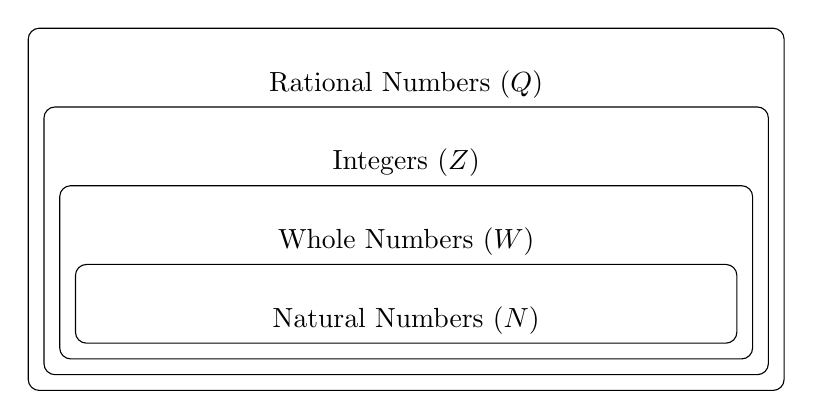
\begin{tikzpicture}
\foreach \x in {1,2,3,4}
	\draw[rounded corners] (-4-\x/5,0.2-\x/5) rectangle (4+\x/5,\x);
\draw (0,0.2) node[anchor=base] {Natural Numbers ($\mathbb{N}$)};
\draw (0,1.2) node[anchor=base] {Whole Numbers ($\mathbb{W}$)};
\draw (0,2.2) node[anchor=base] {Integers ($\mathbb{Z}$)};
\draw (0,3.2) node[anchor=base] {Rational Numbers ($\mathbb{Q}$)};
\end{tikzpicture}
\end{center}